% Options for packages loaded elsewhere
\PassOptionsToPackage{unicode}{hyperref}
\PassOptionsToPackage{hyphens}{url}
%
\documentclass[
]{article}
\usepackage{amsmath,amssymb}
\usepackage{iftex}
\ifPDFTeX
  \usepackage[T1]{fontenc}
  \usepackage[utf8]{inputenc}
  \usepackage{textcomp} % provide euro and other symbols
\else % if luatex or xetex
  \usepackage{unicode-math} % this also loads fontspec
  \defaultfontfeatures{Scale=MatchLowercase}
  \defaultfontfeatures[\rmfamily]{Ligatures=TeX,Scale=1}
\fi
\usepackage{lmodern}
\ifPDFTeX\else
  % xetex/luatex font selection
\fi
% Use upquote if available, for straight quotes in verbatim environments
\IfFileExists{upquote.sty}{\usepackage{upquote}}{}
\IfFileExists{microtype.sty}{% use microtype if available
  \usepackage[]{microtype}
  \UseMicrotypeSet[protrusion]{basicmath} % disable protrusion for tt fonts
}{}
\makeatletter
\@ifundefined{KOMAClassName}{% if non-KOMA class
  \IfFileExists{parskip.sty}{%
    \usepackage{parskip}
  }{% else
    \setlength{\parindent}{0pt}
    \setlength{\parskip}{6pt plus 2pt minus 1pt}}
}{% if KOMA class
  \KOMAoptions{parskip=half}}
\makeatother
\usepackage{xcolor}
\usepackage{longtable,booktabs,array}
\usepackage{calc} % for calculating minipage widths
% Correct order of tables after \paragraph or \subparagraph
\usepackage{etoolbox}
\makeatletter
\patchcmd\longtable{\par}{\if@noskipsec\mbox{}\fi\par}{}{}
\makeatother
% Allow footnotes in longtable head/foot
\IfFileExists{footnotehyper.sty}{\usepackage{footnotehyper}}{\usepackage{footnote}}
\makesavenoteenv{longtable}
\usepackage{graphicx}
\makeatletter
\def\maxwidth{\ifdim\Gin@nat@width>\linewidth\linewidth\else\Gin@nat@width\fi}
\def\maxheight{\ifdim\Gin@nat@height>\textheight\textheight\else\Gin@nat@height\fi}
\makeatother
% Scale images if necessary, so that they will not overflow the page
% margins by default, and it is still possible to overwrite the defaults
% using explicit options in \includegraphics[width, height, ...]{}
\setkeys{Gin}{width=\maxwidth,height=\maxheight,keepaspectratio}
% Set default figure placement to htbp
\makeatletter
\def\fps@figure{htbp}
\makeatother
\setlength{\emergencystretch}{3em} % prevent overfull lines
\providecommand{\tightlist}{%
  \setlength{\itemsep}{0pt}\setlength{\parskip}{0pt}}
\setcounter{secnumdepth}{-\maxdimen} % remove section numbering
\ifLuaTeX
  \usepackage{selnolig}  % disable illegal ligatures
\fi
\usepackage[]{natbib}
\bibliographystyle{plainnat}
\IfFileExists{bookmark.sty}{\usepackage{bookmark}}{\usepackage{hyperref}}
\IfFileExists{xurl.sty}{\usepackage{xurl}}{} % add URL line breaks if available
\urlstyle{same}
\hypersetup{
  pdftitle={Growing Senses: Sense-Specific Developmental World Models of Infant Perception},
  pdfauthor={Somesh (Developmental World Models project)},
  hidelinks,
  pdfcreator={LaTeX via pandoc}}

\title{Growing Senses: Sense-Specific Developmental World Models of
Infant Perception}
\usepackage{etoolbox}
\makeatletter
\providecommand{\subtitle}[1]{% add subtitle to \maketitle
  \apptocmd{\@title}{\par {\large #1 \par}}{}{}
}
\makeatother
\subtitle{Phase-0 technical report}
\author{Somesh (Developmental World Models project)}
\date{14 October 2026}

\begin{document}
\maketitle

\begin{quote}
\textbf{Status.} End-of-day report on the first day of the project. It
combines the minimal models trained in the repository
(\href{https://github.com/pikulsomesh/developmental-world-models}{github.com/pikulsomesh/developmental-world-models})
with three companion analyses done the same day: the paper framing, how
to model age, and how to compare senses fairly. Every experiment here is
a small CPU-scale model on synthetic data. The results are evidence
about \textbf{design choices}, not about infants. Citation keys are
those of \texttt{refs.bib} (\texttt{{[}@key{]}} becomes
\texttt{\textbackslash{}citep\{key\}} in LaTeX), and all references
still need checking before submission.
\end{quote}

\hypertarget{abstract}{%
\section{Abstract}\label{abstract}}

Human infants learn models of their world from a small amount of
experience, received once and in order, through senses that start
immature and come online at different times. We ask which of these
constraints matter for self-supervised world models, and build the
smallest system that can test them: \textbf{one predictive world model
per sense} (vision, hearing, touch, proprioception) in a synthetic
multisensory nursery, each fed through an age-indexed simulation of
sensory immaturity, read out at checkpoints that stand for 0, 3, 6 and
12 months, and combined by a fusion world model. Six training regimes
separate the input schedule from capacity growth and data order. Across
this and two companion toy studies, four results are consistent. (1)
\textbf{The input schedule, not network size, produces the infant-like
trajectory.} With newborn-quality input, vision cannot localise a toy at
the 0- and 3-month checkpoints (probe R² ≈ 0.0) and becomes good by 12
months (0.86), while touch and proprioception are near their mature
level from the start. Growing the network on top of this only slows
learning (0.80 at 12 months). (2) \textbf{Early immaturity buys
robustness at a small cost.} Models raised on immature input lose less
when tested on newborn-quality input than adult-input models (vision
probe R² −0.24 vs −0.40, a noisy difference), and in hearing they
localise better even on clean input (0.45 vs 0.37, consistent over three
seeds). (3) \textbf{Combining senses helps exactly where one sense
fails.} A fused model tracks a toy through a long occlusion better than
the vision model's own memory or hearing alone (hidden-toy position R²
0.77 vs 0.64 and 0.48 at 12 months, three seeds). (4) \textbf{Decodable
is not the same as expected.} No vision model is surprised when an
occluded toy fails to reappear, even when its position is decodable; the
fused model is surprised, but almost entirely through hearing (the toy
stops sounding). Object permanence therefore has to be tested with
paradigms, not probes. We close with the design for the full study:
experience-matched checkpoints of one continuous run per sense,
sensory-immaturity and plasticity schedules as the main levers, capacity
growth as an ablation, late fusion, and perceptual narrowing as the
flagship cross-sense test.

\hypertarget{introduction}{%
\section{1. Introduction}\label{introduction}}

By their first birthday, infants expect unsupported objects to fall and
hidden objects to persist, attribute goals to agents, and have tuned
their perception to the faces and speech sounds around them
\citep{spelke2007core, baillargeon1985object, werker1984cross, pascalis2002species}.
They do this from a few thousand waking hours of egocentric, repetitive
experience, seen once and in order \citep{smith2018curriculum}.
Self-supervised models can now learn useful representations from a
single child's headcam footage
\citep{orhan2020self, orhan2024learning, vong2024grounded}, and
intuitive-physics expectations can emerge from video prediction alone
\citep{garrido2025intuitive}. The sharper question is whether
\textbf{the way infants receive their data matters}.

Infant learning differs from standard training in four documented ways.
The senses start immature \citep{banks1988optical, norcia1985spatial}.
They come online in a fixed order, touch first, hearing before birth and
vision at birth \citep{gottlieb1971ontogenesis}, which may reduce
competition between them \citep{turkewitz1982limitations}. Plasticity is
staggered across senses and levels
\citep{hensch2005critical, werker2015critical}, and synapses are
overproduced and then pruned rather than neurons added
\citep{huttenlocher1997regional}. And experience is a single
non-stationary stream \citep{smith2018curriculum}. Training on initially
blurred or achromatic input can make networks more robust
\citep{vogelsang2018potential, vogelsang2024impact}, slowly changing
early-infant video helps self-supervised learning
\citep{sheybani2023curriculum}, and deep networks have their own
critical periods, including for multisensory integration
\citep{achille2019critical, kleinman2023critical}. But ``starting
small'' \citep{elman1993learning} did not replicate elsewhere
\citep{rohde1999language}, curricula rarely help in standard regimes
\citep{wu2021curricula}, and stage-like learning can arise from learning
dynamics alone \citep{saxe2019mathematical}.

We therefore treat developmental constraints as \textbf{hypotheses to
test rather than design choices to assume}. The source proposal for this
project added object-permanence, agent and goal modules at 4, 6 and 9
months; anything gated that way ``emerges'' on schedule by construction.
Here no module or loss is gated by age, and every capability has to be
measured.

\textbf{Contributions of this phase.}

\begin{enumerate}
\def\labelenumi{\arabic{enumi}.}
\tightlist
\item
  An open, CPU-scale framework with a synthetic multisensory world,
  age-indexed front ends for four senses, sense-specific world models
  with function-preserving growth, and a fusion world model (§3).
\item
  A six-regime comparison that separates sensory immaturity, capacity
  growth and data order, per sense (§4.1--4.2).
\item
  Evidence that fusion carries information through occlusion that no
  single sense keeps, and that decodability and surprise come apart
  (§4.3--4.4).
\item
  A synthesis with two companion studies on age modelling and
  cross-sense comparison (§4.5) and a concrete design for the full study
  (§6).
\end{enumerate}

\hypertarget{related-work}{%
\section{2. Related work}\label{related-work}}

\textbf{Reverse-engineering infant learning.} Programmatic papers argue
that infant learning should be modelled as constrained self-supervised
learning and benchmarked against children
\citep{dupoux2018cognitive, zaadnoordijk2022lessons, cusack2024helpless, smith2017developmental, frank2023bridging, lake2017building}.

\textbf{Learning from a child's perspective.} Headcam corpora
\citep{sullivan2021saycam, long2024babyview} support self-supervised
vision \citep{orhan2020self, orhan2024learning, zhuang2022how} and
grounded word learning \citep{vong2024grounded}, also in a single
chronological pass \citep{jiang2026babycl}; infant-view statistics make
better training data than adult views
\citep{bambach2018toddler, sheybani2023curriculum}.

\textbf{Sensory immaturity and critical periods.} Initial blur
\citep{vogelsang2018potential} and achromatic input
\citep{vogelsang2024impact} benefit later recognition. Critical periods
arise in deep networks
\citep{achille2019critical, kleinman2024critical}, also for multisensory
integration \citep{kleinman2023critical}, and loss of plasticity
parallels their closure \citep{dohare2024loss}.

\textbf{World models and network growth.} We use the predictive
world-model formulation \citep{ha2018world, hafner2023mastering} at toy
scale, a spatial-broadcast decoder \citep{watters2019spatial}, and
function-preserving widening in the spirit of Net2Net
\citep{chen2016net2net} and progressive networks
\citep{rusu2016progressive}.

\textbf{Intuitive physics, agents and brains.} Violation-of-expectation
benchmarks
\citep{riochet2021intphys, weihs2022benchmarking, piloto2022intuitive, gandhi2021baby, stojnic2023commonsense}
and infant fMRI
\citep{deen2017organization, kosakowski2022selective, odoherty2026infants, odoherty2025models}
are the Phase-2 and Phase-4 targets. Multisensory development is framed
by intersensory redundancy \citep{bahrick2000intersensory}. Embodied
touch and proprioception will come from MIMo \citep{mattern2023mimo}.

\hypertarget{framework}{%
\section{3. Framework}\label{framework}}

\begin{figure}
\centering
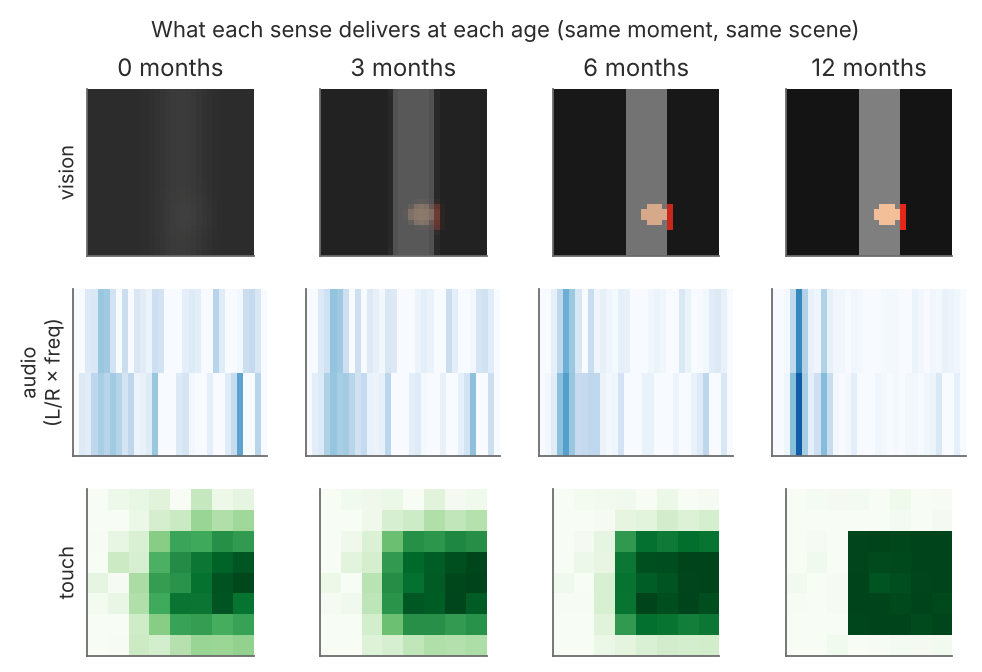
\includegraphics[width=0.8\textwidth,height=\textheight]{figures/fig_senses_by_age.png}
\caption{Figure 1}
\end{figure}

\emph{Figure 1. What each sense delivers at 0, 3, 6 and 12 months, at
the same moment of the same scene. The hand covers the toy in vision,
while touch still feels its shape.}

\hypertarget{a-synthetic-multisensory-nursery}{%
\subsection{3.1 A synthetic multisensory
nursery}\label{a-synthetic-multisensory-nursery}}

One toy of four types moves and bounces in a 32×32 scene; the infant's
own hand babbles in the lower half (\texttt{dwm/env.py}). Each toy type
is specified redundantly across senses \citep{bahrick2000intersensory}:
a shape and colour in \textbf{vision}; a pitch in \textbf{hearing} (2
ears × 32 frequency bins, louder when near, panned by horizontal
position, passing through occluders); a shape on an 8×8 \textbf{tactile}
patch when the hand touches it; and \textbf{proprioception} reports the
hand's position and velocity. Half the scenes contain a vertical
occluder. Two probe sets are generated separately:
\emph{violation-of-expectation} episodes, in which the toy crosses a
central occluder and in the impossible version vanishes while hidden
(from every sense), and \emph{long-occlusion} episodes (occluder 14 px
wide, about 6.6 hidden frames), used to ask where a model thinks the
hidden toy is.

\hypertarget{age-indexed-sensory-front-ends}{%
\subsection{3.2 Age-indexed sensory front
ends}\label{age-indexed-sensory-front-ends}}

Each sense passes through a fixed, non-learned filter whose parameters
are interpolated from per-sense tables (\texttt{dwm/capability.py};
Table 1). Vision uses the proposal's acuity and contrast tables, with
two corrections: contrast sensitivity is applied as a log-compressed
gain rather than a linear one (a linear gain leaves a newborn 2\% of
contrast), and colour starts at 0.1 rather than fully achromatic.
Hearing, touch and proprioception values are coarse placeholders chosen
to respect the known order of maturation (touch and proprioception near
mature at birth, hearing partly, vision far behind).

\begin{longtable}[]{@{}
  >{\raggedright\arraybackslash}p{(\columnwidth - 8\tabcolsep) * \real{0.2000}}
  >{\raggedright\arraybackslash}p{(\columnwidth - 8\tabcolsep) * \real{0.2000}}
  >{\raggedright\arraybackslash}p{(\columnwidth - 8\tabcolsep) * \real{0.2000}}
  >{\raggedright\arraybackslash}p{(\columnwidth - 8\tabcolsep) * \real{0.2000}}
  >{\raggedright\arraybackslash}p{(\columnwidth - 8\tabcolsep) * \real{0.2000}}@{}}
\caption{Per-sense developmental parameters at the four checkpoints.
\{\#tbl:params\}}\tabularnewline
\toprule\noalign{}
\begin{minipage}[b]{\linewidth}\raggedright
Sense
\end{minipage} & \begin{minipage}[b]{\linewidth}\raggedright
0 months
\end{minipage} & \begin{minipage}[b]{\linewidth}\raggedright
3 months
\end{minipage} & \begin{minipage}[b]{\linewidth}\raggedright
6 months
\end{minipage} & \begin{minipage}[b]{\linewidth}\raggedright
12 months
\end{minipage} \\
\midrule\noalign{}
\endfirsthead
\toprule\noalign{}
\begin{minipage}[b]{\linewidth}\raggedright
Sense
\end{minipage} & \begin{minipage}[b]{\linewidth}\raggedright
0 months
\end{minipage} & \begin{minipage}[b]{\linewidth}\raggedright
3 months
\end{minipage} & \begin{minipage}[b]{\linewidth}\raggedright
6 months
\end{minipage} & \begin{minipage}[b]{\linewidth}\raggedright
12 months
\end{minipage} \\
\midrule\noalign{}
\endhead
\bottomrule\noalign{}
\endlastfoot
Vision: acuity (cpd) / contrast sensitivity / colour & 1 / 2 / 0.1 & 4 /
10 / 0.7 & 15 / 50 / 1.0 & 30 / 100 / 1.0 \\
Hearing: frequency blur (bins) / high-frequency pass / binaural
difference & 2.5 / 60\% / 0.3 & 1.8 / 75\% / 0.5 & 1.0 / 90\% / 0.8 &
0.5 / 100\% / 1.0 \\
Touch: receptive-field blur (taxels) / noise & 1.2 / 0.06 & 0.9 / 0.04 &
0.6 / 0.03 & 0.3 / 0.02 \\
Proprioception: position noise & 0.12 & 0.08 & 0.05 & 0.02 \\
Capacity (growing models only): width × / memory window & ×1 / 1 & ×2 /
2 & ×3 / 4 & ×4 / 6 \\
\end{longtable}

\hypertarget{sense-specific-world-models}{%
\subsection{3.3 Sense-specific world
models}\label{sense-specific-world-models}}

Each sense has the same model family (\texttt{dwm/models.py}): an
encoder maps an observation to a latent \(z_t\) (32 dimensions for
vision, 16 for hearing and touch, 8 for proprioception); a residual MLP
predicts \(\hat z_{t+1}\) from the last \(k\) latents and the infant's
motor command; a decoder maps latents back to observations. The loss is
reconstruction of \(o_t\), prediction of \(o_{t+1}\) from
\(\hat z_{t+1}\), and a small latent-consistency term. The vision
encoder is a 3-layer CNN with coordinate channels and the decoder is a
spatial-broadcast decoder \citep{watters2019spatial}; vision losses
up-weight pixels that change between frames, which stands in for
infants' orienting to motion and without which the small toy is ignored.
Other senses use 2-layer MLPs.

\textbf{Growth.} \texttt{grow(width,\ window)} widens every hidden layer
and lengthens the memory window. New units get random incoming and zero
outgoing weights; new memory slots get zero input weights. The grown
model computes exactly the same function as before (unit-tested), then
keeps learning. Vision grows from 44k to 586k parameters and hearing
from 14k to 149k.

\hypertarget{training-regimes}{%
\subsection{3.4 Training regimes}\label{training-regimes}}

Every sense model is trained in one continuous run of four stages (2,000
updates per stage for vision, 1,500 for the other senses) and read out
at the end of each stage; a stage is a checkpoint, not a separate model.

\begin{longtable}[]{@{}
  >{\raggedright\arraybackslash}p{(\columnwidth - 6\tabcolsep) * \real{0.2500}}
  >{\raggedright\arraybackslash}p{(\columnwidth - 6\tabcolsep) * \real{0.2500}}
  >{\raggedright\arraybackslash}p{(\columnwidth - 6\tabcolsep) * \real{0.2500}}
  >{\raggedright\arraybackslash}p{(\columnwidth - 6\tabcolsep) * \real{0.2500}}@{}}
\caption{Training regimes. All see the same data and the same number of
updates. \{\#tbl:regimes\}}\tabularnewline
\toprule\noalign{}
\begin{minipage}[b]{\linewidth}\raggedright
Regime
\end{minipage} & \begin{minipage}[b]{\linewidth}\raggedright
Size
\end{minipage} & \begin{minipage}[b]{\linewidth}\raggedright
Input quality across the four stages
\end{minipage} & \begin{minipage}[b]{\linewidth}\raggedright
Question
\end{minipage} \\
\midrule\noalign{}
\endfirsthead
\toprule\noalign{}
\begin{minipage}[b]{\linewidth}\raggedright
Regime
\end{minipage} & \begin{minipage}[b]{\linewidth}\raggedright
Size
\end{minipage} & \begin{minipage}[b]{\linewidth}\raggedright
Input quality across the four stages
\end{minipage} & \begin{minipage}[b]{\linewidth}\raggedright
Question
\end{minipage} \\
\midrule\noalign{}
\endhead
\bottomrule\noalign{}
\endlastfoot
\textbf{Immature input} (primary) & fixed (12-month size) & 0 → 3 → 6 →
12 months & sensory immaturity alone \\
Immature input + growth & grows ×1 → ×4 & 0 → 3 → 6 → 12 & both levers
(the proposal's idea) \\
Growth only & grows & adult throughout & capacity alone \\
Adult input & fixed & adult throughout & standard ML baseline \\
Shuffled input quality & fixed & each batch drawn from a random stage &
order vs variety \\
Reversed immaturity & fixed & 12 → 6 → 3 → 0 & does the direction
matter? \\
\end{longtable}

\hypertarget{read-outs}{%
\subsection{3.5 Read-outs}\label{read-outs}}

\begin{itemize}
\tightlist
\item
  \textbf{Linear probes} (ridge regression) from a sense model's latent
  to the toy's position (R²) and identity (accuracy; chance 0.25),
  fitted and tested on adult-quality input; touch is probed on contact
  frames and proprioception on the hand's position.
\item
  \textbf{Robustness}: the same probes fitted on adult-quality input and
  tested on newborn-quality input.
\item
  \textbf{Violation of expectation (VoE)}: surprise is one-step
  prediction error at the moment the toy should re-emerge and the next
  two frames; VoE index
  \(= (S_\text{impossible} - S_\text{possible}) / (S_\text{impossible} + S_\text{possible})\),
  positive when the model expects the toy back.
\item
  \textbf{Fusion} (\texttt{dwm/fusion.py}): frozen sense latents are
  projected to a shared space, averaged over the senses present, mixed
  by an MLP into a fused state \(f_t\), and a windowed dynamics model
  predicts \(f_{t+1}\); read-out heads reconstruct every sense latent
  from \(f_t\) and from the prediction. Each sense is dropped at random
  30\% of the time during training. We measure \textbf{cross-modal
  fill-in} (toy position from \(f_t\) with vision switched off) and
  \textbf{occluded tracking} (the hidden toy's horizontal position,
  probed on fully hidden frames; probes fitted on half the episodes,
  tested on the other half).
\end{itemize}

Seeds: three for the four main regimes (and for fusion), one for the
shuffled and reversed controls. Bands and error bars are ±1 s.d. over
seeds where n \textgreater{} 1.

\hypertarget{results}{%
\section{4. Results}\label{results}}

\hypertarget{the-input-schedule-carries-age-growth-only-slows-learning}{%
\subsection{4.1 The input schedule carries age; growth only slows
learning}\label{the-input-schedule-carries-age-growth-only-slows-learning}}

\begin{figure}
\centering
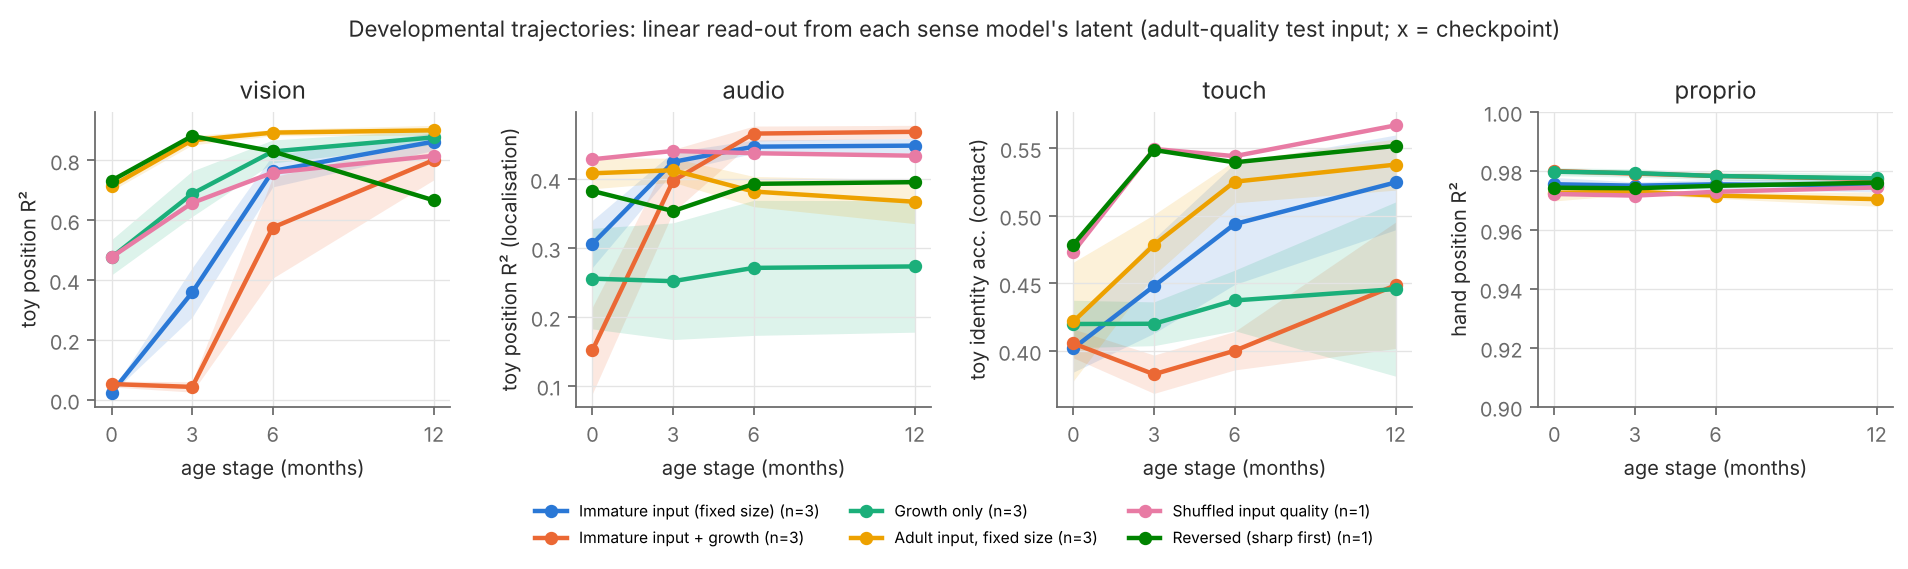
\includegraphics{figures/fig_trajectories.png}
\caption{Figure 2}
\end{figure}

\emph{Figure 2. Developmental trajectories per sense and regime. Each
point is a checkpoint of one continuous run, probed on adult-quality
input.}

With immature input, the vision model cannot localise the toy at the 0-
and 3-month checkpoints (position R² \textbf{0.02} and \textbf{0.36})
and then rises steeply (\textbf{0.77}, \textbf{0.86 ± 0.03}; Figure 2).
The same network trained on adult-quality input localises it at the
first checkpoint (\textbf{0.71}) and ends highest (\textbf{0.90 ±
0.02}). Hearing, touch and proprioception show much flatter curves,
because their front ends start closer to maturity: proprioception is at
ceiling throughout (hand-position R² ≈ 0.97), touch identity accuracy
stays low in every regime (0.40--0.55; the hand rarely covers the whole
toy), and hearing localisation rises from 0.31 to 0.45 as binaural cues
mature. \textbf{The infant order of maturity (body senses first, hearing
next, vision last) appears, and it is put there by the front-end
tables}, which is what the companion cross-sense study also found
(§4.5).

Adding growth on top of immature input does not change this shape; it
\textbf{delays} it. The grown vision model stays at chance through the
3-month checkpoint (0.04) and ends below the fixed-size model
(\textbf{0.80 ± 0.07} vs \textbf{0.86 ± 0.03} position R², \textbf{0.50}
vs \textbf{0.67} identity accuracy). Growth without immature input
(growth only) learns quickly and ends near the adult-input model (0.88).
This matches the age-modelling study (§4.5): capacity changes the speed,
not the shape.

\hypertarget{early-immaturity-buys-robustness-and-in-hearing-it-also-helps-on-clean-input}{%
\subsection{4.2 Early immaturity buys robustness, and in hearing it also
helps on clean
input}\label{early-immaturity-buys-robustness-and-in-hearing-it-also-helps-on-clean-input}}

\begin{figure}
\centering
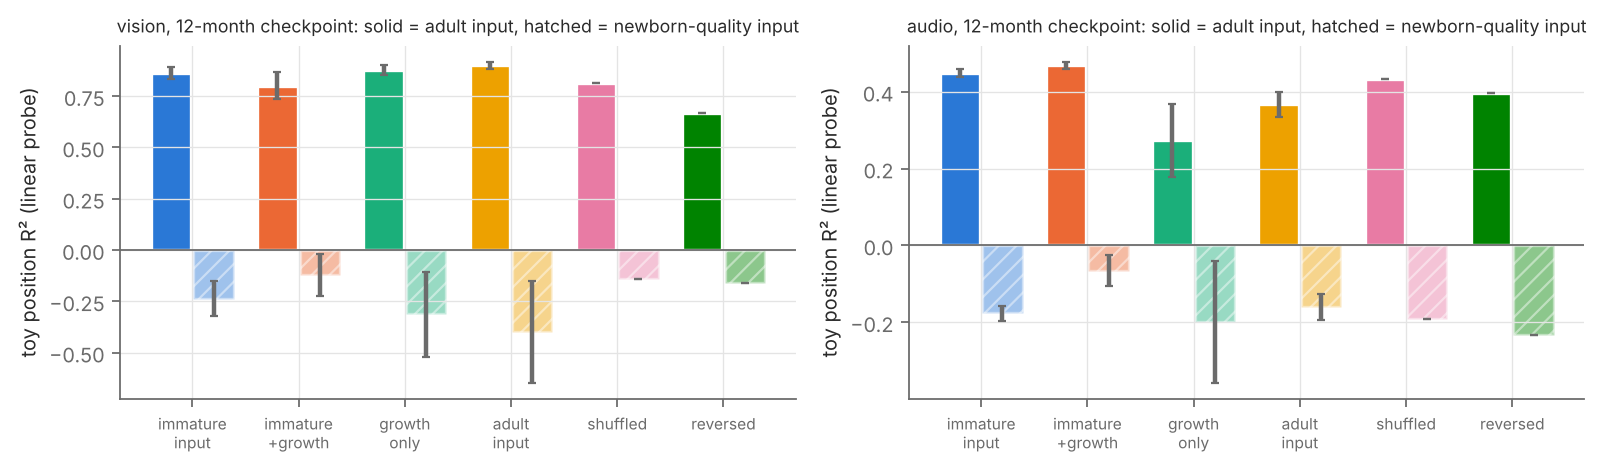
\includegraphics{figures/fig_robustness.png}
\caption{Figure 3}
\end{figure}

\emph{Figure 3. Probes at the 12-month checkpoint on adult-quality input
(solid) and newborn-quality input (hatched).}

On clean input, adult-input vision is best (Figure 3). On
\textbf{newborn-quality} input, every regime that ever saw immature
input degrades less on average: probe R² \textbf{−0.24 ± 0.08} (immature
input), \textbf{−0.12 ± 0.10} (immature + growth), \textbf{−0.14}
(shuffled) and \textbf{−0.16} (reversed), against \textbf{−0.40 ± 0.25}
for adult input and \textbf{−0.31 ± 0.21} for growth only. The
adult-input seeds vary a lot, and all values are negative (worse than
guessing the mean), so this is ``less bad'' rather than robust; the
direction matches blur-first training in classifiers
\citep{vogelsang2018potential} and the age-modelling study's
blur-robustness result.

Hearing goes further. Models that saw immature hearing early localise
better \textbf{on clean input} at 12 months (position R² \textbf{0.45 ±
0.01} immature, \textbf{0.47 ± 0.01} immature + growth) than models that
only heard adult-quality sound (\textbf{0.37 ± 0.03} adult input,
\textbf{0.27 ± 0.10} growth only). Shuffled (0.43) and reversed (0.40)
quality are in between, so for hearing the benefit seems to come from
having seen degraded input at all, a form of augmentation, more than
from its order. This is the one place in our data where a developmental
constraint improves clean performance. It holds in all three seeds, but
the hearing front end is a placeholder, so it is a lead to test with
real audio rather than a claim.

Reversed immaturity is the clearest negative control: the vision model
that ends on newborn-quality input loses what it had (0.88 at the second
checkpoint, \textbf{0.67} at the last). Order matters in the obvious
direction.

\hypertarget{combining-senses-fusion-keeps-what-each-sense-loses}{%
\subsection{4.3 Combining senses: fusion keeps what each sense
loses}\label{combining-senses-fusion-keeps-what-each-sense-loses}}

\begin{figure}
\centering
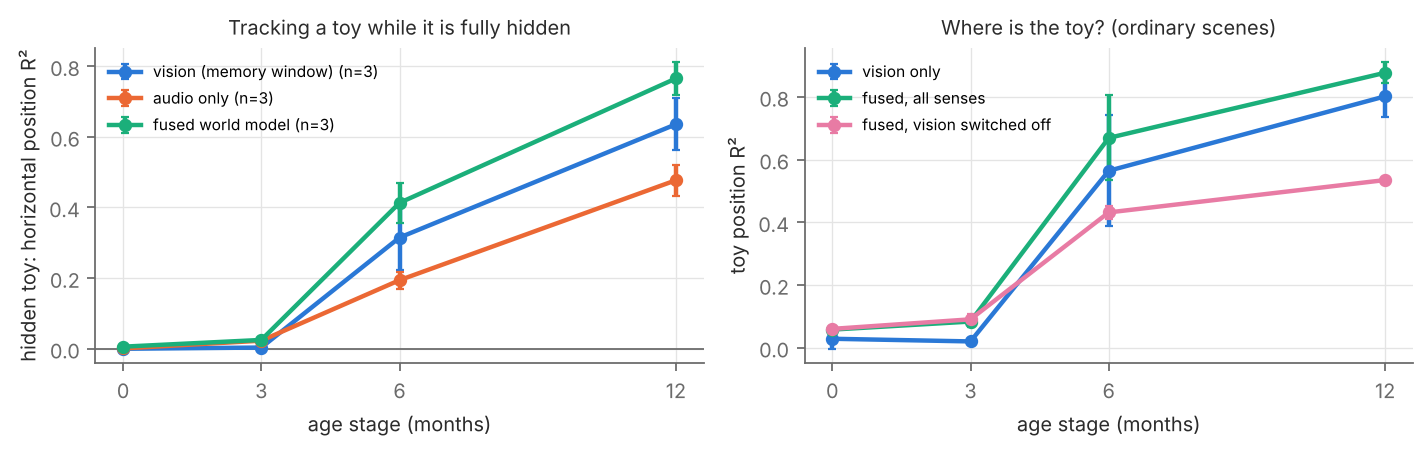
\includegraphics{figures/fig_fusion.png}
\caption{Figure 4}
\end{figure}

\emph{Figure 4. Left: horizontal position of a fully hidden toy, decoded
from the vision model's memory window, from hearing alone, and from the
fused world model. Right: toy position in ordinary scenes from vision
alone, from the fused state, and from the fused state with vision
switched off.}

During a long occlusion the hidden toy's horizontal position is
decodable from the vision model's memory window (R² \textbf{0.64 ± 0.07}
at 12 months), from hearing, which passes through the occluder
(\textbf{0.48 ± 0.04}), and best from the fused world model
(\textbf{0.77 ± 0.05}; Figure 4, left). The fusion advantage appears at
6 months (0.41 vs 0.31 and 0.19) and nothing is decodable at 0--3
months, when neither vision nor binaural hearing can localise. In
ordinary scenes, the fused state is better than vision alone (0.88 ±
0.03 vs 0.80 ± 0.07) and, with vision switched off, still recovers
position from hearing, touch and the hand (0.53; Figure 4, right). Toy
identity is trivially available from pitch in hearing (accuracy 1.0 at
every age), so the fused model inherits it, while vision alone reaches
only 0.50--0.74 depending on regime. This supports the design that
trains each sense separately and fuses later, which the age-modelling
study found preserves the best per-sense encoders (§4.5).

\hypertarget{decodable-is-not-expected-object-permanence-must-be-tested-as-surprise}{%
\subsection{4.4 Decodable is not expected: object permanence must be
tested as
surprise}\label{decodable-is-not-expected-object-permanence-must-be-tested-as-surprise}}

\begin{figure}
\centering
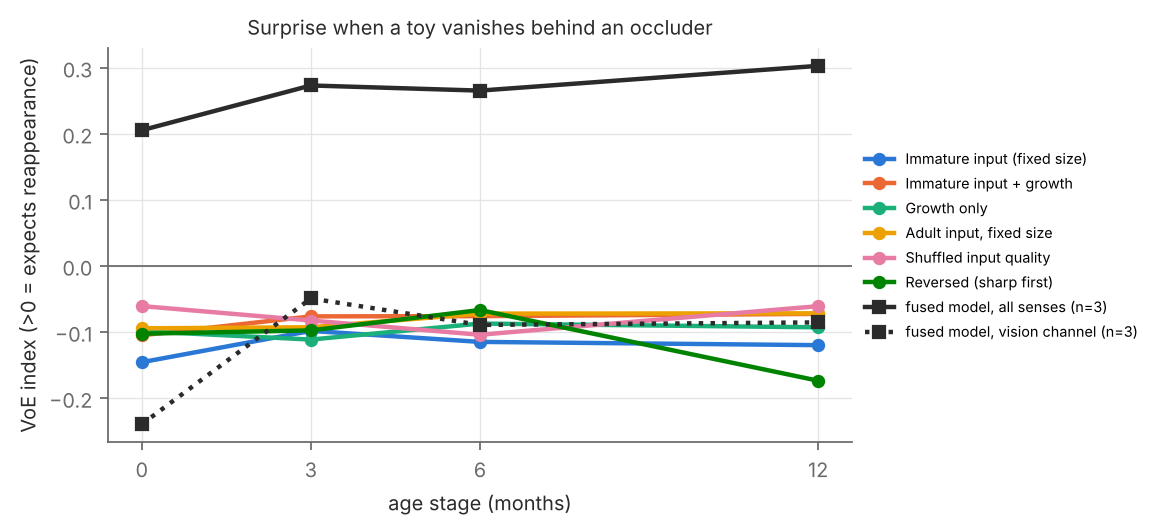
\includegraphics{figures/fig_voe.png}
\caption{Figure 5}
\end{figure}

\emph{Figure 5. VoE index when the toy vanishes behind an occluder:
unimodal vision models in every regime (coloured) and the fused world
model (black), overall and through its vision channel only.}

No vision model in any regime shows a positive VoE index (all between
\textbf{−0.17} and \textbf{−0.06}; Figure 5): they are \emph{more}
surprised when the toy reappears than when it fails to. They behave like
a ``copy the last frame'' predictor, even though the toy's hidden
position is decodable from the same model's memory (§4.3). The fused
world model does show a positive index that grows with age (\textbf{0.21
± 0.02} at 0 months to \textbf{0.30 ± 0.08} at 12), but decomposing its
surprise by sense shows that it comes from \textbf{hearing} (audio
channel 0.43 → 0.75; vision channel −0.24 → −0.09): in our impossible
events the toy vanishes from every sense, so the fused model notices
that the sound stopped. Its vision channel stays negative, like the
unimodal models. Two conclusions follow. First, a probe can show that
information about a hidden object is present while the model's
predictions do not use it; infant-style paradigms are needed to claim
permanence. Second, multisensory VoE needs events that dissociate the
senses (for example, a toy that vanishes visually but keeps sounding, or
a silent toy) before it says anything about visual permanence.

\hypertarget{companion-studies}{%
\subsection{4.5 Companion studies}\label{companion-studies}}

Two toy studies run in parallel used independent code and stimuli and
point the same way.

\textbf{How to model age} (\texttt{research/age-modeling/}). In small
CNNs on a shape-versus-texture task, the proposal's acuity schedule
alone produced the infant-like curve (near chance, then a coarse-shape
phase, then a jump to fine detail at about 6 months), whatever the
capacity strategy; growing the network was slowest and never fully
learned the fine cue (texture-only 0.66 vs 0.91). A run that went
through the blurry months ended more shape-sensitive and more
blur-robust than a separate 12-month model trained only on 12-month
input, which has no history. Most strikingly, \textbf{the same three
months of blur caused a lasting deficit only when they came first}
(fine-detail accuracy after recovery 0.81 for months 0--3, against
0.94--1.00 for later windows): a critical period in a plain continuous
run with no plasticity schedule \citep{achille2019critical}. In a
two-sense version, the sense that came online first crowded out the
later one under joint training (the vision encoder ended at 0.60 vs 0.84
for vision alone in the human, hearing-first order), and training each
sense separately before fusing gave the best per-sense encoders at a
small fused-accuracy cost (0.88 vs 0.91)
\citep{kleinman2023critical, turkewitz1982limitations}.

\begin{figure}
\centering
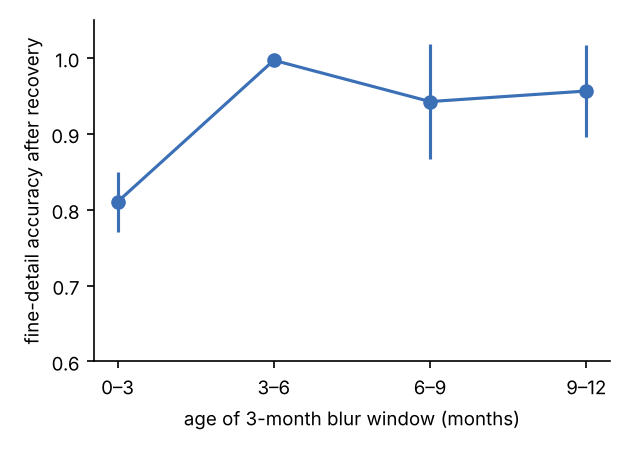
\includegraphics[width=0.6\textwidth,height=\textheight]{figures/e2b_window.png}
\caption{Figure 6}
\end{figure}

\emph{Figure 6. Age-modelling study: a 3-month blur window placed at
different ages, each followed by 8 months of clear input.}

\textbf{How to compare senses fairly} (\texttt{research/cross-sense/}).
With one latent world rendered into vision, hearing and touch, and
violations applied to the latent, five world-model families at matched
core size gave: front ends alone reproduce the order of maturity at
birth (vision hidden-object R² −2.23 at birth vs 0.33 at 12 months;
touch 0.38 vs 0.32); \textbf{memory is the only requirement shared by
all senses} (the memoryless model was last on VoE in every sense), while
the ranking of other families changes by sense; the objective decides
what a model notices (a JEPA-style latent predictor tracked hidden
objects best in vision but was nearly blind to identity changes in
sound); extra capacity did not rescue newborn vision; and, importantly,
\textbf{perceptual narrowing emerged without being built in}: trained
only on two ``native'' identities, vision surprise at a never-seen
contrast rose to 0.54 and then fell to 0.29 while the native contrast
reached 1.18, and hearing narrowed in its representation (d′ 5.19 →
1.33) without showing surprise.

\begin{figure}
\centering
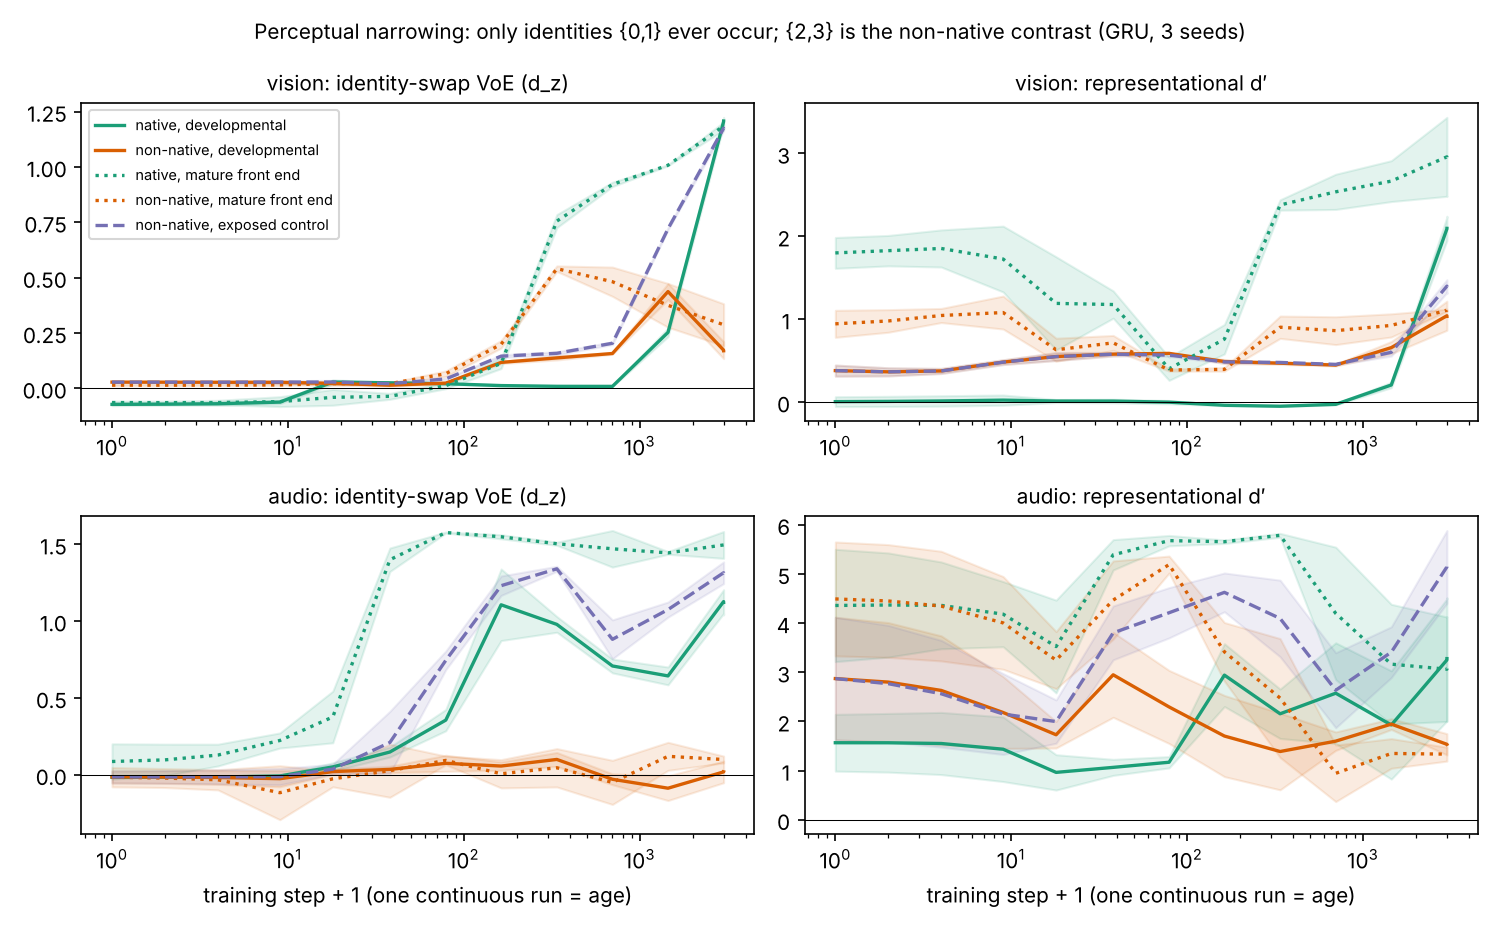
\includegraphics[width=0.8\textwidth,height=\textheight]{figures/narrowing.png}
\caption{Figure 7}
\end{figure}

\emph{Figure 7. Cross-sense study: perceptual narrowing in one
continuous run per model; ``non-native'' identities are never seen in
training.}

\hypertarget{discussion}{%
\section{5. Discussion}\label{discussion}}

\textbf{What carries age.} Three independent toy settings agree that the
infant-like shape of development comes from the \textbf{input schedule},
and that growing the network mostly slows learning. This is consistent
with neurobiology, where neurons are not added after birth but the
periphery, synapse density, myelination and plasticity change on
per-sense clocks
\citep{huttenlocher1997regional, sydnor2021neurodevelopment, hensch2005critical}.
Capacity should be a controlled factor and not the definition of age;
separate per-age models cannot express the history effects (critical
periods, robustness from early blur) that a continuous run shows.

\textbf{What the constraints buy.} The costs and benefits are specific.
Immature early vision costs a little on clean input and buys some
robustness; immature early hearing improved clean localisation here.
Neither is a free lunch, which is the honest version of ``starting
small'' \citep{elman1993learning, rohde1999language} and the reason the
full study must report both sides.

\textbf{Why sense-specific models, then fusion.} Senses mature on
different clocks, differ in what their front ends can deliver, and
compete when trained jointly. Training each sense on its own schedule
and fusing later keeps each encoder at its best and still gives the
fused model information no single sense has (tracking through
occlusion). The cross-sense study adds that the fusion and sense models
should share one family with memory.

\textbf{Limitations.} Everything is synthetic, small (at most 0.6M
parameters), and evaluated with linear probes and one VoE paradigm. The
newborn vision filter is harsh at 32×32 (the toy is barely visible), and
hearing, touch and proprioception tables are placeholders. ``Months''
are stages of 1,500--2,000 updates, not experience hours. Seeds are few
(three for the main regimes, one for the order controls), and the
robustness ordering in vision is within seed noise. The VoE result for
fusion is driven by hearing because our impossible events remove the toy
from every sense.

\hypertarget{toward-the-full-study-and-the-arxiv-paper}{%
\section{6. Toward the full study and the arXiv
paper}\label{toward-the-full-study-and-the-arxiv-paper}}

Combining today's results with the framing note
(\texttt{research/paper-framing.md}):

\begin{enumerate}
\def\labelenumi{\arabic{enumi}.}
\tightlist
\item
  \textbf{Age = experience.} One continuous run per sense, one
  chronological pass, checkpoints at cumulative waking hours for 0, 1,
  2, 3, 4, 6, 9, 12 (18, 24) months.
\item
  \textbf{Main levers}: per-sense sensory immaturity (real visual-angle
  optics, a womb low-pass filter for prenatal hearing) and a bottom-up
  plasticity schedule. \textbf{Factors}: capacity (fixed, grown,
  overproduce-then-prune), data order (chronological, shuffled,
  reversed), sense onset order.
\item
  \textbf{One model family with memory for every sense}; report one
  reconstruction-based and one latent-prediction (JEPA-style) model.
\item
  \textbf{Late fusion} after sense-specific training, with onset order
  as a factor.
\item
  \textbf{Evaluation = the capability matrix as tests}: VoE, habituation
  and preferential looking, with dissociating multisensory events;
  metrics for order (Kendall τ against infant milestones), timing and
  shape; \textbf{perceptual narrowing as the flagship cross-sense test};
  age-matched neural alignment later \citep{odoherty2026infants}.
\item
  \textbf{Data path}: synthetic (done) → MIMo for touch and
  proprioception \citep{mattern2023mimo} → SAYCam/BabyView for vision
  and hearing \citep{sullivan2021saycam, long2024babyview}.
\item
  \textbf{Paper}: framed as a test of which constraints are necessary or
  sufficient for which signatures, with pre-registered predictions.
  Suggested title: \emph{Growing Up Sensory: Testing Which Developmental
  Constraints Make Self-Supervised World Models Infant-Like}. Primary
  category cs.LG, cross-listed to q-bio.NC.
\end{enumerate}

\textbf{Reproducibility.} \texttt{scripts/queue.sh} runs the full grid;
\texttt{scripts/make\_figures.py} and
\texttt{scripts/analyze\_fusion\_voe.py} regenerate every figure from
\texttt{results/}. Companion code is in the project folder
(\texttt{research/age-modeling/code},
\texttt{research/cross-sense/xsense}).

\renewcommand\refname{References}
  \bibliography{refs.bib}

\end{document}
